%% bare_jrnl.tex
%% V1.4b
%% 2015/08/26
%% by Michael Shell
%% see http://www.michaelshell.org/
%% for current contact information.
%%
%% This is a skeleton file demonstrating the use of IEEEtran.cls
%% (requires IEEEtran.cls version 1.8b or later) with an IEEE
%% journal paper.
%%
%% Support sites:
%% http://www.michaelshell.org/tex/ieeetran/
%% http://www.ctan.org/pkg/ieeetran
%% and
%% http://www.ieee.org/


\documentclass[journal]{IEEEtran}


\usepackage{times}
\usepackage{epsfig}
\usepackage{graphicx}
\graphicspath{{images/}}
\usepackage[justification=centering]{caption}
\usepackage{subfigure}
\usepackage{float} %插图
\usepackage{mathtools}
\usepackage{amsmath}
\usepackage{amssymb}
\usepackage{multirow}
\usepackage{cite}
\usepackage{bm}%公式文本粗体
\usepackage{hyperref}
\usepackage{xfrac}% 斜分�?\usepackage{booktabs}%表格
\usepackage{array}% 表格

\usepackage{algorithm}
\usepackage{algpseudocode}
\renewcommand{\algorithmicrequire}{\textbf{Input:}}  % Use Input in the format of Algorithm
\renewcommand{\algorithmicensure}{\textbf{Output:}} % Use Output in the format of Algorithm
\newcommand{\initial}{\textbf{Initial:}}
% 算法
\makeatletter
\newcommand{\rmnum}[1]{\romannumeral #1}
\newcommand{\Rmnum}[1]{\expandafter\@slowromancap\romannumeral #1@}
\makeatother



% correct bad hyphenation here
\hyphenation{op-tical net-works semi-conduc-tor}


\begin{document}

\title{Small Target Detection in Infrared Videos \\Based on Spatio-Temporal Tensor Model}
%
%
% author names and IEEE memberships
% note positions of commas and nonbreaking spaces ( ~ ) LaTeX will not break
% a structure at a ~ so this keeps an author's name from being broken across
% two lines.
% use \thanks{} to gain access to the first footnote area
% a separate \thanks must be used for each paragraph as LaTeX2e's \thanks
% was not built to handle multiple paragraphs
%

\author{Hong-Kang~Liu,~Lei~Zhang,~\IEEEmembership{Member,~IEEE}
        and~Hua~Huang,~\IEEEmembership{Member,~IEEE}% <-this % stops a space
\thanks{H.-K. Liu, L. Zhang and H. Huang were with the School of Computer, Beijing Institute of Technology, Beijing, 100081 China. E-mail: leizhang@bit.edu.cn}% <-this % stops a space
}

% note the % following the last \IEEEmembership and also \thanks -
% these prevent an unwanted space from occurring between the last author name
% and the end of the author line. i.e., if you had this:
%
% \author{....lastname \thanks{...} \thanks{...} }
%                     ^------------^------------^----Do not want these spaces!
%
% a space would be appended to the last name and could cause every name on that
% line to be shifted left slightly. This is one of those "LaTeX things". For
% instance, "\textbf{A} \textbf{B}" will typeset as "A B" not "AB". To get
% "AB" then you have to do: "\textbf{A}\textbf{B}"
% \thanks is no different in this regard, so shield the last } of each \thanks
% that ends a line with a % and do not let a space in before the next \thanks.
% Spaces after \IEEEmembership other than the last one are OK (and needed) as
% you are supposed to have spaces between the names. For what it is worth,
% this is a minor point as most people would not even notice if the said evil
% space somehow managed to creep in.



% The paper headers
\markboth{IEEE Transactions on Geoscience and Remote Sensing,~Vol.~xx, No.~x, xxxx~2019}%
{Shell \MakeLowercase{\textit{et al.}}: Bare Demo of IEEEtran.cls for IEEE Journals}
% The only time the second header will appear is for the odd numbered pages
% after the title page when using the twoside option.
%
% *** Note that you probably will NOT want to include the author's ***
% *** name in the headers of peer review papers.                   ***
% You can use \ifCLASSOPTIONpeerreview for conditional compilation here if
% you desire.




% If you want to put a publisher's ID mark on the page you can do it like
% this:
%\IEEEpubid{0000--0000/00\$00.00~\copyright~2015 IEEE}
% Remember, if you use this you must call \IEEEpubidadjcol in the second
% column for its text to clear the IEEEpubid mark.



% use for special paper notices
%\IEEEspecialpapernotice{(Invited Paper)}




% make the title area
\maketitle

% As a general rule, do not put math, special symbols or citations
% in the abstract or keywords.
\begin{abstract}
Existing methods of the small target detection from infrared videos are not effective with the highly complex background. It is mainly caused by: i) the interference of strong edges and the similarity with other non-target components; ii) the lack of the context information of both the background and the target in the spatio-temporal domain. By considering these two points, we propose to slide a window in a single image and form a spatio-temporal cube with the current image patch and other image patches in the spatio-temporal domain. Then, we establish a spatio-temporal tensor model based on the patches. According to the sparse prior of the target and the local correlation of the background, the separation of the target and the background can be cast as a low-rank and sparse tensor decomposition problem. The target image is reconstructed from the sparse tensor obtained by the tensor decomposition. The experiments show that our method gains better detection performance in infrared videos with highly complex background, by making full use of the context information in the spatio-temporal domain.
\end{abstract}

% Note that keywords are not normally used for peerreview papers.
\begin{IEEEkeywords}
Infrared video, small target detection, spatio-temporal tensor model, tensor decomposition.
\end{IEEEkeywords}


%Intruction
%
%

\section{Introduction}

\IEEEPARstart{A}{t} present, the infrared target detection technology has been widely used in missile tracking, precision guidance, early warning, maritime surveillance, ground monitoring~\cite{luo2015space,dawson2010space,li2014infrared}, \emph{etc}. Compared with the ordinary detection task, the lack of sufficient information to distinguish the target is the main challenge of the small target detection for infrared videos. Due to the long infrared imaging distance, the size of small targets in infrared videos is very small, generally ranging from $2\times2$ to $9\times9$ pixels~\cite{wang2017infrared}. And in the case of the long imaging distance, the small target in infrared videos has no regular shape and texture features. In addition, the infrared radiation of the target is heavily attenuated after the long distance propagation, which results in a low signal-to-noise ratio (SNR) for small infrared targets~\cite{li2016novel}. When there are complex background clutter and noise, the small target with low signal-to-clutter ratio (SCR) is usually buried in the background. Therefore, the detection of small targets in the complex infrared background remains a challenging problem.

Compared with visible videos, infrared videos looks simpler. However, the infrared video lacks color and texture information, and has poor image quality, which causes great difficulty in processing the small target. Concretely, the lack of color information will result in fewer features for distinguishing the target from the background, while the lack of texture and shape information means that the target cannot be distinguished based on some feature learning methods directly. Therefore, it is necessary to use the motion characteristics of the target as well as the relationship between the small target and the background to detect infrared small targets.

The small target detection methods for infrared videos are classified into two categories: single-frame detection methods based on only the spatial information and spatio-temporal detection methods based on both inter-frame temporal information and intra-frame spatial information~\cite{li2016novel}. Generally, the small target on a single frame is invisible by the perception and it is impossible to distinguish the target by using only the information in the spatial domain. Contrarily, it is important to make full use of the context information of the small target in the temporal domain. The current spatio-temporal detection methods usually calculate the local contrast of spatial domain and temporal domain separately, and combine them to detect the small target. Obviously, only calculating the local contrast can not distinguish the true small target in the case of complex noise or motion of the background, which results in excessive false and missed alarms. In order to make full use of the effective information in both the temporal and spatial domain, we propose a method for small target detection based on the spatio-temporal tensor decomposition.

The main contribution of this paper is a spatio-temporal tensor model that considers the local correlation of background image patches in both the spatial and temporal domain. This can suppress the background clutter well. Actually, our method not only delivers the spatial salience of the target, but also makes full use of the motion characteristic in the temporal domain by utilizing the sparse prior of the small target.
This enables a better performance of the infrared small target detection than some state-of-the-art methods.

The remain of this paper is organized as follows. Section~\Rmnum{2} presents the related research in the field of the infrared small target detection. In Section \Rmnum{3}, we propose the spatio-temporal tensor model and our method for detecting infrared small targets by the spatio-temporal tensor decomposition. Section \Rmnum{4} gives the experiments to verify the effectiveness of our method. Section \Rmnum{5} concludes this paper and discusses the future work.

%Related work
%
%
\section{Related Work}

We briefly review the related work on the infrared small target detection methods based on single image and multiple images, which correspond to single frame detection and spatio-temporal detection for infrared videos.

\subsection{Detection Methods Based on Single Image}

The methods for target detection based on the single image have two types, which are established on two assumptions. One type assumes the background changes slowly in the infrared image, and the high correlation exists between adjacent pixels. The other type utilizes the non-local self-correlation between background patches in the infrared image, which assumes that all background image patches in the infrared image are from a low rank subspace or a mixed set composed of multiple low rank subspaces~\cite{liu2013robust}.

For the first type, many filtering-based methods are proposed, e.g., two-dimensional least mean square( TDLMS) filter~\cite{hadhoud1988two}, max-median and max-mean filter~\cite{deshpande1999max}, transform domain methods \cite{davidson2002wavelet,peng2004dim} and so on. This type of methods enhance the small target by calculating the difference between the original image and the predicted background. Some other filter-based methods exploit the mechanism of the human visual system, e.g., the Laplacian of Gaussian (LoG) filter \cite{kim2009small}, the difference of Gaussian (DoG) \cite{wang2012infrared} and the second-order directional derivative~\cite{qi2013robust}. Although this type of methods can reduce the influence of edges compared with traditional methods, it can not suppress clutters and strong edges in the complex background. This results in many false alarms. Meanwhile, there is usually a large difference between the infrared small target and its surrounding background, by which some methods use the local contrast measure (LCM)~\cite{chen2014local}, the improved local contrast measure (ILCM)~\cite{han2014robust}, the multi-scale patch-based contrast measure (MPCM) \cite{wei2016multiscale} and so on. Alternatively, other methods based on the local difference measure (LDM) \cite{deng2017entropy}, the local saliency map (LSM) \cite{chen2016efficient} and the weighted local difference measure (WLDM) \cite{deng2016small} have also been proposed. Generally, these methods can suppress the background and enhance the small target, but a large amount of noise and clutters might also be enhanced in the case of the complex background, which are considered as small targets with the high false alarm rate.

For the second type, the small target detection in the infrared image can be transformed into a low rank matrix recovery problem. Gao \emph{et al}.~\cite{gao2013infrared} propose to convert the separation of the target and the background into a matrix recovery problem. Then, the target could be separated from the background by recovering the low rank and sparse matrices. However, this method still has bad effect in the face of strong edges and clutters. RIPT~\cite{dai2017reweighted} extracts prior features by the local structure information, and then suppress edges with the local structure weight in the process of the small target detection. But in the case of the complex background, background patches may come from multiple low rank subspaces, so Wang \emph{et al}.~\cite{wang2017infrared} use the multiple subspace learning strategy to suppress background, which can reduce the false alarm rate effectively. The above methods are based on the robust principal component analysis (RPCA) to achieve the small target detection. However, due to the existence of many clutters in the background in a single image, like cloud patches in the sky and fixed heat objects on the ground, the detection of the true target might be interfered seriously. The information in a single image is not sufficient to distinguish the small target, so it is necessary to take the temporal information into account.

\subsection{Detection Methods Based on Multiple Images}

By using multiple images, it can make full use of the spatial information to suppress background clutters and the temporal information to highlight the small target, which benefits the detection accuracy. The recursive variance filter (TVF)~\cite{silverman1998temporal} and the damped sinusoid filter (TTF)~\cite{caefer1998temporal} are proposed to detect the small target from multiple images. However, the difference of the target and the moving background can not be distinguished according to only the temporal information. For example, the moving cloud might also be detected as the target. Therefore, Deng \emph{et al}.~\cite{deng2016infrared} propose a spatio-temporal local contrast filter (STLCF) for the infrared small target detection. But the calculation of the local contrast is prone to be affected by the noise. Gao \emph{et al}. propose TVPCF~\cite{gao2017tvpcf} that combines the multi-scale local contrast based on patches with the temporal filter to obtain better detection results. Li \emph{et al}.~\cite{li2016novel} propose to use image patches in the spatio-temporal neighborhood of the current image patch to reconstruct a new image patch. Then, the difference between the current image patch and the reconstructed image patch is defined as the spatio-temporal local contrast for the target detection. Although this method can suppress clutters and the single pixel noise, the reconstruction is extremely sensitive to the noise. In this case, many targets might be lost under the high noise.

\begin{figure*}[htb]
  \centering
  \includegraphics[width=0.9\textwidth]{flowchart.pdf}
  \caption{The work flow of our small target detection based on the spatio-temporal tensor model.}
  \label{fig:flow_chart}
\end{figure*}


\section{Construction and Decomposition of the Spatio-temporal Tensor Model}

The key ingredient for our small target detection setup is a spatio-temporal tensor model built on the stack of patches.
As shown in Figure~\ref{fig:flow_chart}, each frame is segmented into patches by sliding a window with the prescribed size, and a patch cube is formed by stacking the current patch and the ones from the adjacent patches in the spatial and temporal domain. Then, the patch cube is viewed as a spatio-temporal tensor, where the background tensor is of low rank and the target tensor is sparse. Therefore, the target patch can be distinguished from all the original patches by separating the target tensor from the original one. Next, we will elaborate the details of constructing and decomposing the spatio-temporal model.


\subsection{Construction of the spatio-temporal tensor model}

Typically, the model for the infrared small target detection is defined as follows \cite{gu2010kernel}:
\begin{equation}
  f_D(x,y)=f_B(x,y)+f_T(x,y)+f_N(x,y)
  \label{eq:image_model}
\end{equation}
where $f_D$, $f_B$, $f_T$ and $f_N$ are the input infrared image, background image, target image and noise image respectively, and $(x,y)$ are the position coordinates of each pixel respectively. 
 
We divide the input frame into a set of patches by sliding a window from top to bottom, and left to right. So each patch of size $ps \times ps$ is extracted. And the sliding step is $ss$. Then, we get $M$ patches ($N_r$ rows and $N_c$ columns)  from the each frame. Then based on Eq.(\ref{eq:image_model}), we have
\begin{equation}
  P_D^h(i,j)=P_B^h(i,j)+P_T^h(i,j)+P_N^h(i,j)
  \label{eq:patch_model}
\end{equation}
where $P_*(i,j)$ denotes the image patch of current frame, $(i,j)$ represents the index of patch, $h$ denotes the index of frame .

We let $c$ denote the index of current frame and $P_D^c(i,j)$ denote current patch in current frame. As shown in Figure \ref{construction}, for patch $P_D^c(i,j)$, we collect image patches from its spatio-temporal local adjacent domain to form a spatio-temporal patch cube. 

Firstly, we constrcut the spatial patch cube with image patches in spatial local neighborhood, such as the blue part in Figure \ref{construction}. In this paper, we choose $m_s=9$ patches (including current patch) in spatial local neighborhood of current patch and the patch indexes of these spatial patches are $(i+u,j+v),u,v \in [-1,1]$. So a spatial patch cube is obtained with all patches $P_D^{c}(i+u,j+v),u,v \in [-1,1]$, and we view it as a spatial patch tensor as follows:
\begin{equation}
  \bm{\mathcal T}_D^s = \bm{\mathcal T}_B^s + \bm{\mathcal T}_T^s + \bm{\mathcal T}_N^s
  \label{eq:spatial_tensor_model}
\end{equation}
where $\bm{\mathcal T}_D^s$, $\bm{\mathcal T}_B^s$, $\bm{\mathcal T}_T^s$, $\bm{\mathcal T}_N^s \in {\mathbb R}^{{I}\times{J}\times{m_s}}$ are the tensors composed of the input frame patches, background patches, target patches and noise patches in the spatially adjacent domain respectively. Here, $I$ and $J$ denote the height and the width of each patch, which depends on the size of the sliding window, $m_s$ denotes the number of patches in spatial local adjacent domain.

Next, a temporal patch cube is formed for patch $P_D^c(i,j)$ with patches in its temporal local neighborhood, such as the purple part in Figure \ref{construction}. In this paper, we choose $2*p$ adjacent frames of current frame. Among them, there are $p$ frames before current frame and $p$ frames after current frame, and the frame index of them are $c+q,q\in [-p,p]$. Then, we also choose $m_s=9$ patches in the temporal local neighborhood of each adjacent frame. And the patch indexes of these temporal patches in each adjacent frame are $(i+u,j+v),u,v \in [-1,1]$. So we construct the temporal patch cube with all patches $P_D^{c+q}(i+u,j+v),q\in [-p,-1]\cup[1,p]\text{ and }u,v \in [-1,1]$. We view the temporal patch cube as temporal patch tensor as follows:
\begin{equation}
    \bm{\mathcal T}_D^t = \bm{\mathcal T}_B^t + \bm{\mathcal T}_T^t + \bm{\mathcal T}_N^t 
  \label{eq:temporal_tensor_model}
\end{equation}
 Where $\bm{\mathcal T}_D^t$, $\bm{\mathcal T}_B^t$, $\bm{\mathcal T}_T^t$, $\bm{\mathcal T}_N^t \in {\mathbb R}^{{I}\times{J}\times{m_t}}$ are the tensors composed of the input frame patches, background patches, target patches and noise patches from the temporally adjacent frames respectively. Also, $I$ and $J$ have the same meanings. And $m_t$ denotes the number of patches in temporal local adjacent domain.

 \begin{figure}[H]
  \centering
  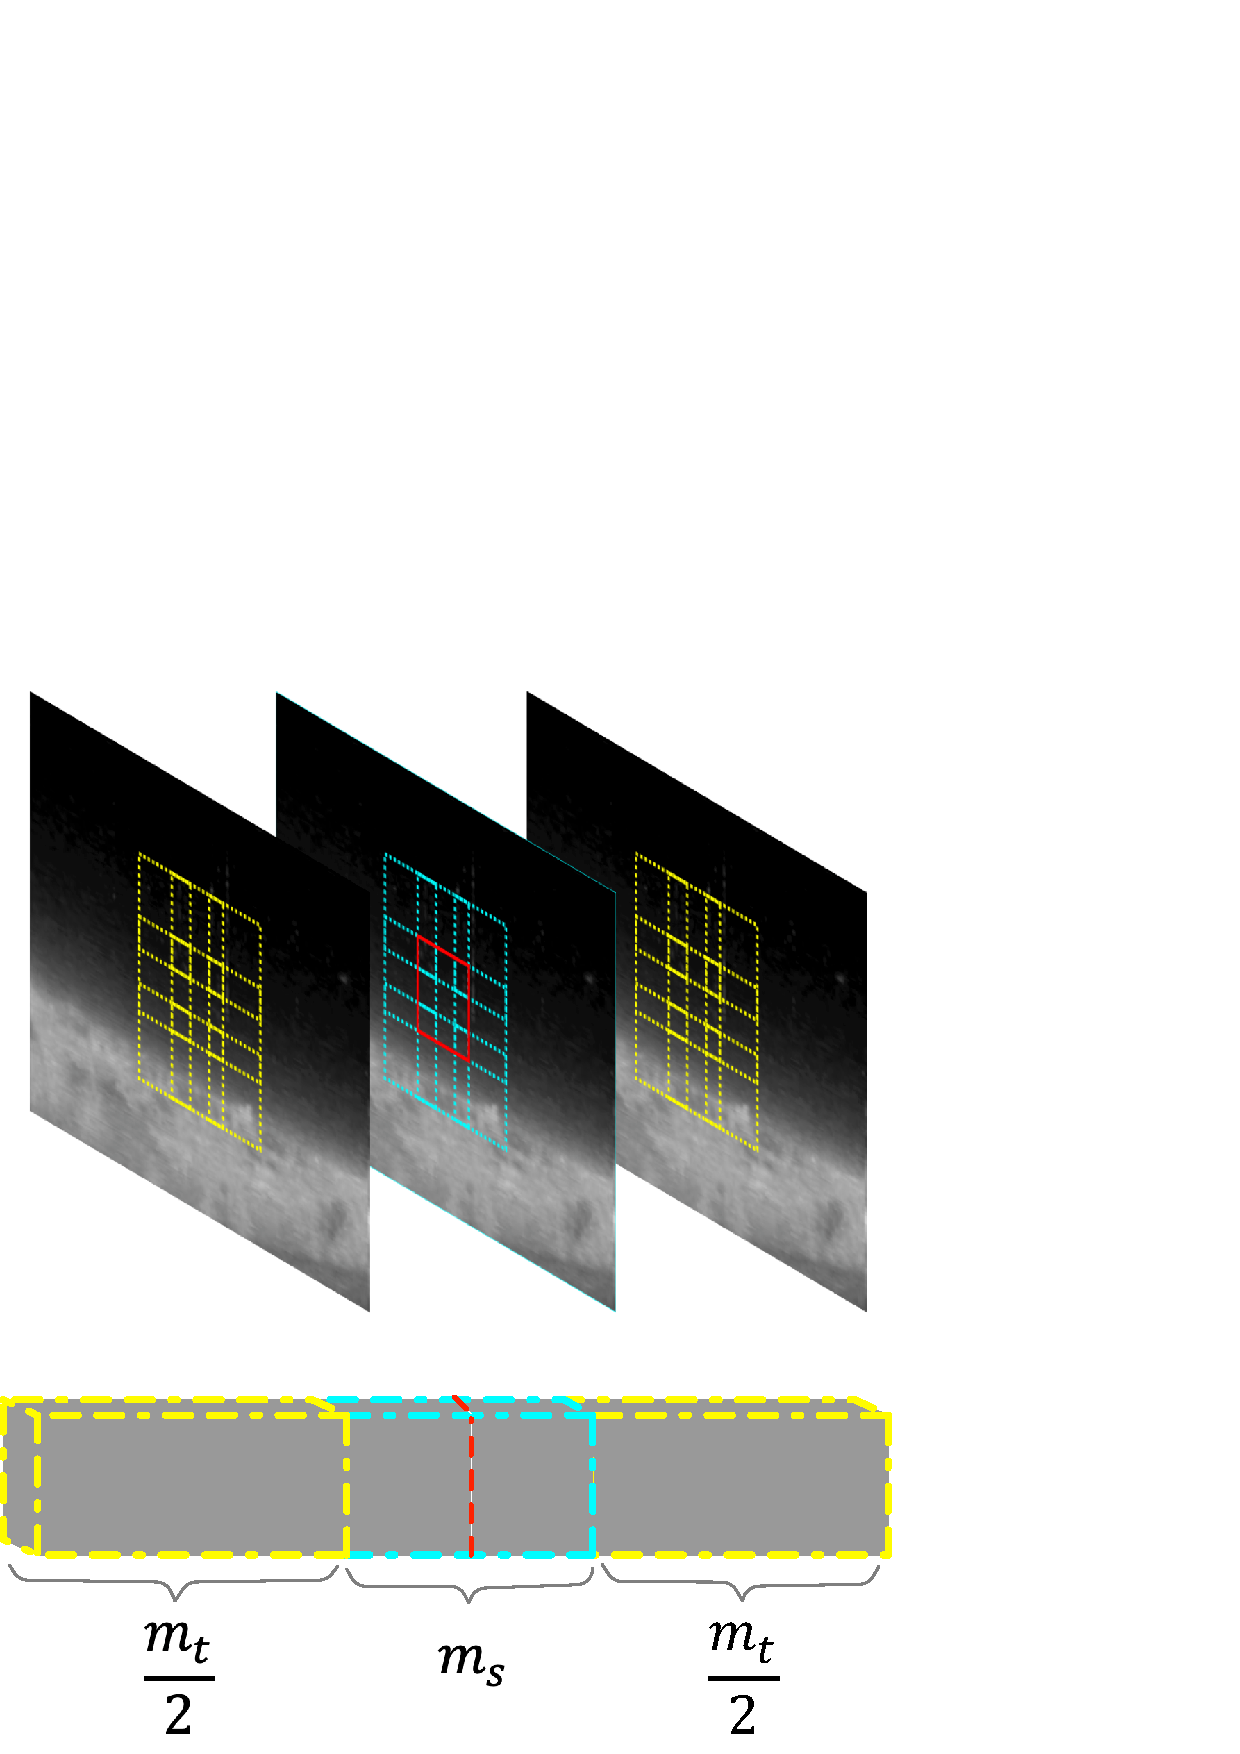
\includegraphics[width=0.45\textwidth]{construction.pdf}
  \caption{The construction of the spatio-temporal patch cube.}
  \label{construction}
\end{figure}

Finally, in order to make full use of the information in spatio-temporal adjacent domain, the spatio-temporal patch cube can be obtained by splicing the spatial and temporal cube as mentioned above, as shown in Figure \ref{construction}. And according to the analysis above, we know that
\begin{equation}
  \bm{\mathcal T}_D^{st} = \bm{\mathcal T}_B^{st} + \bm{\mathcal T}_T^{st} + \bm{\mathcal T}_N^{st}
  \label{eq:spatio_temporal_tensor_model}
\end{equation}
where $\bm{\mathcal T}_D^{st},\bm{\mathcal T}_B^{st},\bm{\mathcal T}_T^{st},\bm{\mathcal T}_N^{st} \in {\mathbb R}^{{I}\times{J}\times{(m_t+m_s)}}$ are the tensors for the adjacent patches in both the spatial and temporal domains. $(m_t+m_s)$ is the total number of the adjacent patches in spatio-temporal domain.

So far, we have constructed the new spatio-temporal tensor model for infrared small target detection task, which makes full use of the information in spatial and temporal domain at the same time. Next, we will analyze the characteristic of three parts in spatio-temporal patch tensor.


\textbf{Background patch tensor $\mathbf{\mathcal T}_B^{st}$.}\quad
There is usually a strong correlation between the spatial adjacent patches in the background in local neighborhood. Besides, the background changes slowly compared to the target, so the background patches also have the strong correlation between adjacent frames in the temporal local domain. Thus, we can employ the low rank property for the background characterization.

\begin{figure}[H]
  \centering
  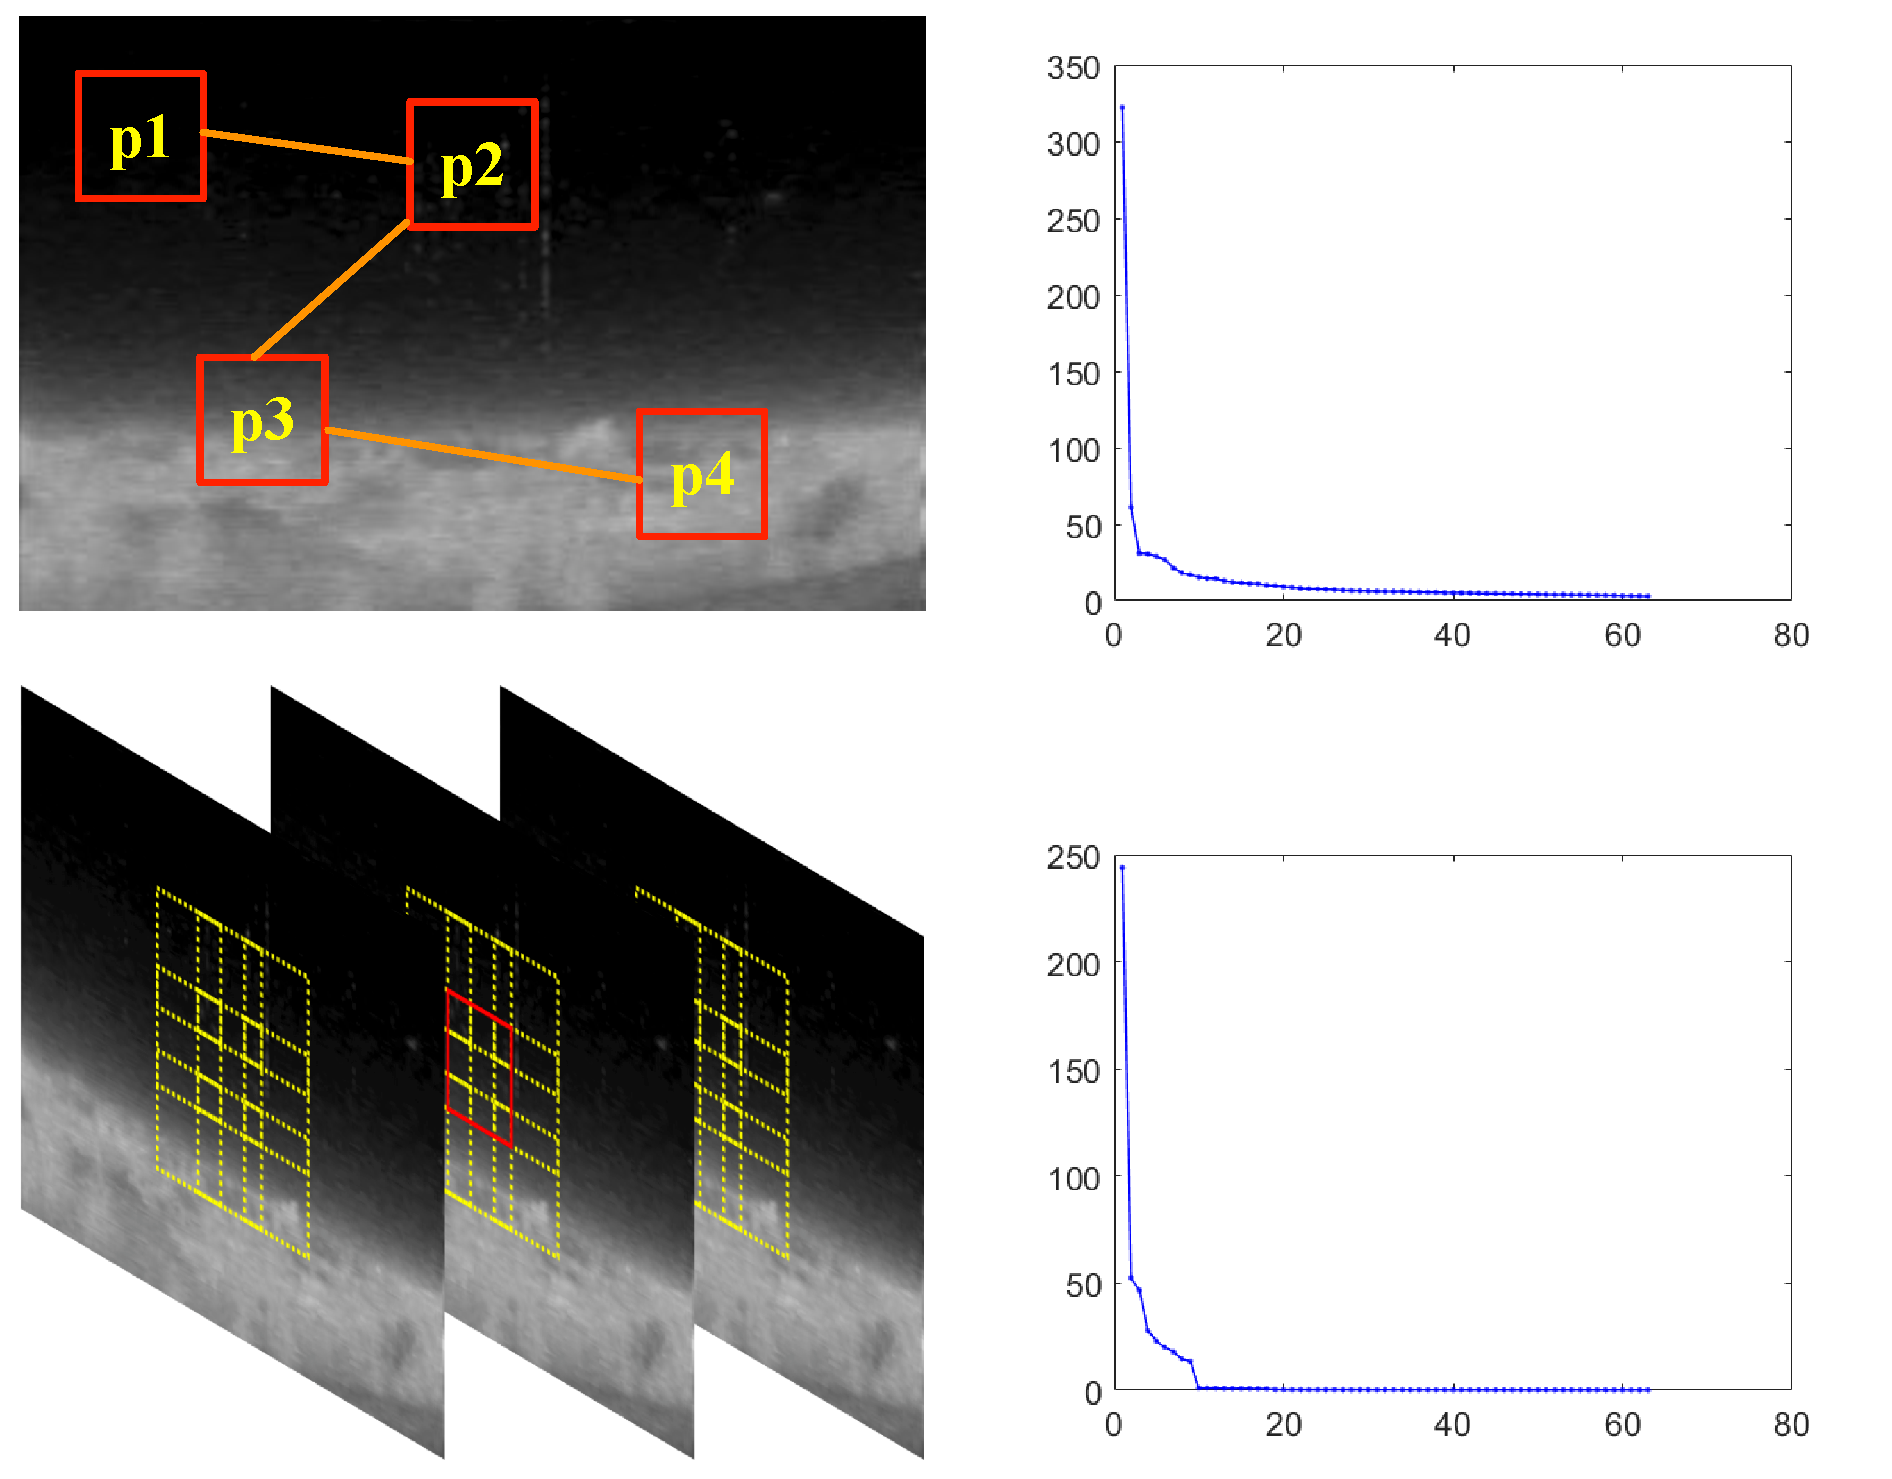
\includegraphics[width=0.45\textwidth]{singular.eps}
  \caption{The singular value distribution of the non-local correlation (\textbf{top}) and the local correlation (\textbf{bottom}).}
  \label{singular}
\end{figure}

Here, we employ the traditional IPI model~\cite{gao2013infrared} to calculate the non-local correlation of background image patches. And we obtained the local correlation of them according to the spatio-temporal cube construction method mentinoed above. In order to compare with traditional IPI model for convenience, our spatio-temporal tensor model selects several background image patches in spatio-temporal adjacent domain, and the IPI model randomly selects same number of background image patches in non-local regions. 

A matrix is attained according to the IPI model, whose one column corresponds to one background patch from non-local regions. Then we get a spatio-temporal tensor based on our spatio-temporal construction method. So we transform it into a mode-1 unfold matrix. And the singular values are calculated of the matrixs formed by two models. It can be seen from the top and bottom of Figure \ref{singular} that the singular values of the spatio-temporal tensor which utilizes the local correlation of background image patches decrease faster. It proves that the background tensor in our model has better low rank characteristics, meanwhile the local correlation of background patches is stronger than non-local. So it can be ensured that the edge and details of background components (clutters) will be preserved during the tensor decomposition process.

Based on the above analysis, it is known that the background  tensor is of low rank, i.e.,
\begin{equation}
  \mbox{rank}(\bm{\mathcal T}_B^{st}) \leq r
\end{equation}
where $r$ is a  constant that constrains the low rank of the background tensor. Usually, $r$ appears to be bigger in the complex background than the uniform background.


\textbf{Target Image Patch Tensor $\mathbf{\mathcal T}_T^{st}$.}\quad
In actual application scenario, due to the infrared imaging characteristics, there is no obvious texture information and color information of small targets in infrared video. And the brightness of infrared small target is also different in different scenes. Moreover, the size of different targets also vary within a certain range. But infrared small targets are always small in size because of that imaging distance is far. So if small target appears in spatio-temporal patch cube, the volume occupied by small target is great small compared with the volume of entire spatio-temporal patch cube. Therefore, the target image patch tensor is a sparse tensor actually, and it satisfies:
\begin{equation}
  \left \| \bm{\mathcal T}_T^{st} \right \|_0 \leq k
\end{equation}
where $k$ is a small constant that can be intuitively regarded as the volume corresponding to target, which is determined by the size of target and the number of times that small target appears in spatio-temporal patch cube.

\textbf{Noise Image Patch Tensor $\mathbf{\mathcal T}_N^{st}$.}\quad
As mentioned in\cite{gao2013infrared}, random noise in infrared video is generally considered to be independent and identically distributed Gaussian white noise. And for a given $\delta>0$, noise image patch tensor satisfies $\left \| \bm{\mathcal T}_N^{st} \right \|_F \leq \delta$. So according to Eq.(\ref{eq:spatio_temporal_tensor_model}), we can get the following restriction:
\begin{equation}
  \left \| \bm{\mathcal T}_D^{st}-\bm{\mathcal T}_B^{st}-\bm{\mathcal T}_T^{st} \right \|_F \leq \delta.
\end{equation}
The $r,k,\delta$ vary in different image patch tensor, but we will not utilize the specific values of them.

Based on the above spatio-temporal tensor model, we can analyze the behaviors of the small target in the spatial and temporal domain simultaneously.
Next, we will solve the model by using the classical low-rank tensor recovery for detecting the small target in infrared videos.

\subsection{The Decomposition Method for Spatio-temporal Image Patch Tensor}
The ultimate goal of us is to detect small target in infrared video, so we need to get target image $f_T$ based on original image $f_D$ given. As shown in figure \ref{fig:flow_chart}(c), the current target patches of all target tensors corresponding to entire original image can be reconstructed to obtain target image, so it is critical to attain target tensor from original spatio-temporal tensor.

We first assume that there is no noise in original infrared image, then original image consists of background image and target image, expressed in the tensor model as $\bm{\mathcal T}_D^{st}=\bm{\mathcal T}_B^{st}+\bm{\mathcal T}_T^{st}$. According to the above discussion, we know that background image patch tensor is low-rank and the target image patch tensor is sparse. So we can attain target image patch tensor and background image patch tensor from tensor decomposition. And then, we can reconstruct target image from all target image patch tensors. Therefore, the original target detection problem is transformed into the following optimization problem according to our model:
\begin{equation}
  \underset{\bm{\mathcal T}_B^{st},\bm{\mathcal T}_T^{st}}{min} \ rank(\bm{\mathcal T}_B^{st}) + \lambda \left \| \bm{\mathcal T}_T^{st} \right \|_0 \ s.t. \bm{\mathcal T}_D^{st}=\bm{\mathcal T}_B^{st}+\bm{\mathcal T}_T^{st}
  \label{min_1}
\end{equation}
But the optimization problem is a NP-hard problem, and it is impossible to calculate the rank of background image patch tensor. Therefore, we adopt nuclear norm $\left \| \bm{\mathcal T}_B^{st} \right \|_*$ to restrict background image patch tensor instead of low-rank constraint. At the same time, in order to facilitate the calculation, we substitute $l_0$ norm with $l_1$ norm of target image patch tensor. Then, we consider that noise tensor satisfies $\left \| \bm{\mathcal T}_N^{st}\right \|_F \leq \delta$. So, the optimization problem in Eq.(\ref{min_1}) can be transformed into following convex optimization problem:
\begin{equation}
  \underset{\bm{\mathcal T}_B^{st},\bm{\mathcal T}_T^{st}}{min} \ \left \| \bm{\mathcal T}_B^{st} \right \|_* + \lambda \left \| \bm{\mathcal T}_T^{st} \right \|_1 \ s.t. \left \|\bm{\mathcal T}_D^{st}-\bm{\mathcal T}_B^{st}-\bm{\mathcal T}_T^{st} \right \|_F\leq \delta
  \label{min_2}
\end{equation}
The $\lambda$ parameter mentioned above plays a balancing role between background tensor and target tensor. The detail for selection of $\lambda$ will be described in next subsection.

Solving the tensor decomposition problem utilizing ADMM algorithm mentinoed in \cite{dai2017reweighted}, the augmented lagrangian expression of the Eq.(\ref{min_2}) can be written as:
\begin{equation}
  \begin{split}
    L & = \left \|\bm{\mathcal T}_B^{st} \right \| _* +\left \|\bm{\mathcal T}_T^{st} \right \| _1 + \\
    & \frac{\alpha}{2} \left \|\bm{\mathcal T}_D^{st}-\bm{\mathcal T}_B^{st}-\bm{\mathcal T}_T^{st} \right \| ^2 - \langle \bm{\mathcal F},\bm{\mathcal T}_D^{st}-\bm{\mathcal T}_B^{st}-\bm{\mathcal T}_T^{st} \rangle
  \end{split}
\end{equation}

\subsection{Optimization}
\subsubsection{Background tensor estimation}
With the other terms fixed, the background tensor $\bm{\mathcal T}_B^{st}$ can be estimated from the following minimization problem:
\begin{equation}
  E(\bm{\mathcal T}_B^{st})=\frac{\alpha}{2} \left \|\bm{\mathcal T}_B^{st}-(\bm{\mathcal T}_D^{st}-\bm{\mathcal T}_T^{st}+\frac{\bm{\mathcal F}}{\alpha}) \right \|_F^2 + \left \|\bm{\mathcal T}_B^{st} \right \| _*
  \label{optimization1}
\end{equation}

Eq.(\ref{optimization1}) can be easily solved by a soft thresholding operation on the singular values of observation tensor~\cite{cai2010singular}:
\begin{equation}
  \begin{dcases}
    \bm{\mathcal J_1}=\bm{\mathcal T}_D^{st}-\bm{\mathcal T}_T^{st}+\frac{\bm{\mathcal F}}{\alpha}\\
    (\bm{\mathcal T}_B^{st})^{k+1}=\bm{U}(shrink\_L_{*}(\Sigma,\frac{1}{\alpha}))\bm{V}^{T}\\
    shrink\_L_{*}(\Sigma,\eta)=max(\Sigma_{ii}-\eta,0)
  \end{dcases}
  \label{opti1}
\end{equation}
In the second step of Eq.(\ref{opti1}), we transform the temporary tensor $\bm{\mathcal J_1}$ into mode-1 unfold matrices $\bm{J_1}$. And $\bm{J_1}=\bm{U}\Sigma\bm{V}^{T}$ is the singular value decomposition of $\bm{J_1}$ and $\Sigma_{ii}$ is the diagonal element of the singular value matrix. After a soft thresholding operation, we convert the metrices obtained into tensor $(\bm{\mathcal T}_B^{st})^{k+1}$.

\subsubsection{Target tensor estimation}
With the other terms fixed, the target tensor $\bm{\mathcal T}_T^{st}$ can be estimated from the following minimization problem:
\begin{equation}
  E(\bm{\mathcal T}_T^{st})=\frac{\alpha}{2} \left \|\bm{\mathcal T}_T^{st}-(\bm{\mathcal T}_D^{st}-\bm{\mathcal T}_B^{st}+\frac{\bm{\mathcal F}}{\alpha}) \right \|_F^2 + \lambda \left \|\bm{\mathcal T}_T^{st} \right \| _1
  \label{optimization2}
\end{equation}
which can be solved efficiently by a soft shrinkage operation:
\begin{equation}
  \begin{dcases}
    \bm{\mathcal J_2}=\bm{\mathcal T}_D^{st}-\bm{\mathcal T}_B^{st}+\frac{\bm{\mathcal F}}{\alpha}\\
    (\bm{\mathcal T}_T^{st})^{k+1}=shrink\_L_{1}(\bm{\mathcal J_2},\frac{\lambda}{\alpha})\\
    shrink\_L_{1}(\xi,\eta)=\frac{\xi}{|\xi|} \ast max(\xi-\eta,0)
  \end{dcases}
  \label{opti2}
\end{equation}

\subsubsection{Update the multiplier and penalization parameter}
\begin{equation}
  \begin{dcases}
    \bm{\mathcal F}^{k+1}=\bm{\mathcal F}^{k}+\alpha^{k}(\bm{\mathcal T}_D^{st}-\bm{\mathcal T}_B^{st}-\bm{\mathcal T}_T^{st})\\
    \alpha^{k+1}=\alpha^{k} \ast \rho
  \end{dcases}
  \label{optimization3}
\end{equation}

Finally, we choose $\lambda=\sfrac{1}{(\sqrt{m_s+m_t}\times ss + ps)}$, $\rho=1.01$.



%�?1 和表 2
\begin{table*}[t]
  \centering
  \caption{scene introduction of simulation video set}
  \label{tab1}
  \begin{tabular}{|c|m{3cm}<{\centering}|m{3cm}<{\centering}|m{3cm}<{\centering}|m{3.2cm}<{\centering}|}
    \hline
    &Seq1 &Seq2 &Seq3 &Seq4\\
    \hline
    representative video frame& 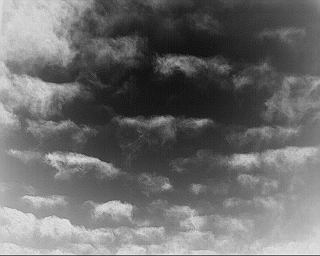
\includegraphics[scale=0.33]{back1.png}& 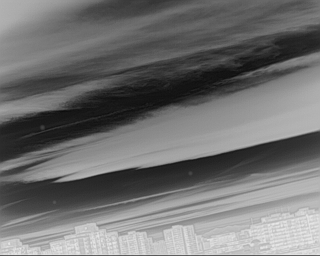
\includegraphics[scale=0.25]{back2.png}& 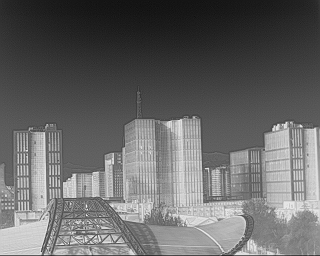
\includegraphics[scale=0.33]{back3.png}& 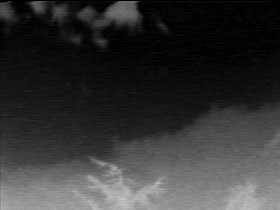
\includegraphics[scale=0.3]{back4.png}\\
    \hline
    size($width \times height$)& $320 \times 256$& $320 \times 256$& $320 \times 256$& $280\times 210$\\
    \hline
    Scene description& Sky scene with complex clouds moving constantly & Sky scene full filled with clouds and some buildings & Complex buildings scene with much interference & Clouds and tree branches are moving quickly due to gale\\
    \hline
    noise level & small & medium & big & big \\
    \hline
    target number & 1 & 3 & 2 & 2 \\
    \hline
  \end{tabular}
\end{table*}

\begin{table*}[t]
  \centering
  \caption{scene introduction of real video set}
  \label{tab2}
  \begin{tabular}{|c|m{3cm}<{\centering}|m{3cm}<{\centering}|m{3cm}<{\centering}|m{3.2cm}<{\centering}|}
    \hline
    &Seq1 &Seq2 &Seq3 &Seq4\\
    \hline
    representative video frame&
    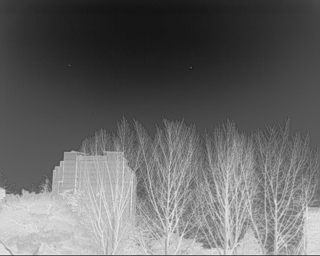
\includegraphics[scale=0.26]{real-back1.png}&
    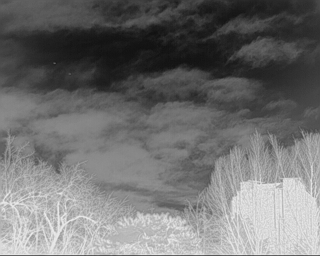
\includegraphics[scale=0.26]{real-back2.png}&
    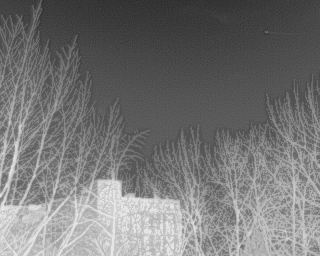
\includegraphics[scale=0.26]{real-back3.png}&
    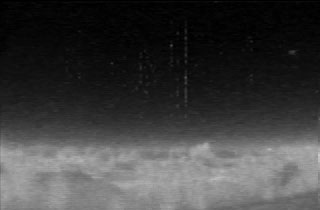
\includegraphics[scale=0.29]{real-back4.png}\\
    \hline
    size($width \times height$)& $320 \times 256$& $320 \times 256$& $320 \times 256$& $320\times 210$\\
    \hline
    Scene description& Sky scene with buildings and trees, no cloud & Sky scene full filled with clouds and trees & Include buildings and tree branches & A single plane gradually disappears behind the horizon\\
    \hline
    noise level & small & medium & big & big \\
    \hline
    target number & 2 & 2 & 1 & 1 \\
    \hline
    target & birds & birds & plane & plane \\
    \hline
  \end{tabular}
\end{table*}


\subsection{The Detection Process Based on Spatio-temporal Tensor Model}
As shown in Figure \ref{fig:flow_chart}, the main process of detection method proposed in this paper is shown in algorithm \ref{algorithm1}.
\begin{algorithm}[H]
  \caption{The Detection Algorithm Based on Spatio-temporal Tensor Model}
  \begin{algorithmic}[1]
    \Require
    current frame $f_D^c$, adjacent frames $f_D^{c+q},q\in \left [-p,-1 \right]\cup \left [1,p \right ]$
    \State
    \initial   $\quad ss=15,\ ps=80,\ \epsilon>0$
    \State $N_r*N_c$ image patches obtained, initial $i=1,j=1$
    \While{$(i<=N_r) \ and \ (j<=N_c)$}
    \State Form $\bm{\mathcal T}_D^{st}$ according to subsection A 
    \State
    \initial   $\quad k=0,\ (\bm{\mathcal T}_T^{st})^{0}=\bm{0}, \ (\bm{\mathcal T}_B^{st})^{0}=\bm{\mathcal T}_D^{st}, \ \bm{\mathcal F}^0=\bm{0},\ \alpha^0=\sfrac{1}{mean(S_{[6-10]})}$ where $S_*$ is the $*_{th}$ largest value of $vec(\bm{\mathcal T}_D^{st})$
    \Repeat
    \State Fix the others and update $\bm{\mathcal T}_B^{st}$ by Eq.(\ref{optimization1}) and Eq.(\ref{opti1})
    \State Fix the others and update $\bm{\mathcal T}_T^{st}$ by Eq.(\ref{optimization2}) and Eq.(\ref{opti2})
    \State Update $\bm{\mathcal F}$ and $\alpha$ by Eq.(\ref{optimization3})
    \State Update $k$: $\quad k=k+1$
    \Until{$\frac{\left \| \bm{\mathcal T}_D^{st}-(\bm{\mathcal T}_B^{st})^{k+1}-(\bm{\mathcal T}_T^{st})^{k+1} \right \|_F}{\left \|\bm{\mathcal T}_D^{st} \right \|}<\epsilon $}
    \State Obtain $\bm{\mathcal T}_T^{st}$
    \EndWhile
    \State Aggregate $\bm{\mathcal T}_T^{st}$ to form the target frame $f_T^c$
    \Ensure
    current target frame $f_T^c$
  \end{algorithmic}
  \label{algorithm1}
\end{algorithm}

According to the above detection process, good results can be obtained. And small target in complex background can be accurately detected. In addition, we think that some post-processing methods could improve detection result significantly. But we adopt none post-processing method in our experiment part to compare the advantages and disadvantages of each detection method for infrared small target fairly.


\section{Experiment And Analysis}
In order to reflect the effectiveness and advancement of our mathod, we compare our method with five detection methods of different types in the following experiments. Our method utilizes both spatial and temporal information, so it is firsty compared with three detection methods that only use spatial information, namely MPCM method\cite{wei2016multiscale}, IPI method\cite{gao2013infrared} and RIPT method\cite{dai2017reweighted}. And then, we also compare our method with two detection methods which utilize both spatial and temporal information in infrared video, they are STLCF method\cite{deng2016infrared} and the method proposed by Li et al\cite{li2016novel}(STSA). We analyze the performance of each detection method on different infrared video sets.

\subsection{Measurement Metrics}
The measurement metrics used in our experiments reference the metrics defined in\cite{gao2013infrared}\cite{dai2017reweighted}. But we adjust the scope of adjacent domain of target as $d=40$. The measurement metrics are defined as follows.

Signal-to-clutter ratio (SCR) is one of the most common measurement metrics, usually used to measure the difficulty of small target detection. The calculation formula is defined as follows:
\begin{equation}
  \mbox{SCR}=\frac{\left| \mu_t -\mu_b \right|}{\sigma_b}
  \label{SCR}
\end{equation}
where $\mu_t \text{ and }\mu_b$ are the mean intensity of target domain and background adjacent domain respectively. And $\sigma$ is the standard deviation of background area. According to Eq.(\ref{SCR}), the gain of SCR is defined as:
\begin{equation}
  \mbox{SCR}_{gain}=\frac{\mbox{SCR}_{out}}{\mbox{SCR}_{in}}
\end{equation}
where $\mbox{SCR}_{in}$, $\mbox{SCR}_{out}$ are the $\mbox{SCR}$ values of input infrared image and the output image after detection process.

The second measurement metric is background suppression rate, which is defined as follows:
\begin{equation}
  \mbox{BSF}=\frac{\sigma_{in}}{\sigma_{out}}
\end{equation}
where $\sigma _{in}$ and $\sigma _{out}$ are the standard deviations of background neighborhood in input image and output image. Another metric is the gain of local signal to noise ratio $(\mbox{LSNR}_{gain})$. Firstly, $\mbox{LSNR}$ is defined as $\mbox{LSNR}=\sfrac{I_t}{I_b}$, where $I_t$ and $I_b$ represents the maximum intensity of target area and background neighborhood, respectively. So $\mbox{LSNR}_{gain}$ is defined as:
\begin{equation}
  \mbox{LSNR}_{gain}=\frac{\mbox{LSNR}_{out}}{\mbox{LSNR}_{in}}
\end{equation}

In addition to the above metrics, we also calculated the probablity of detection $P_d$ and false-alarm rate $F_a$, which are defined as follows:
\begin{equation}
  P_d=\frac{\mbox{number\;of\;true\;detections}}{\mbox{number\;of\;actual\;targets}}
\end{equation}
\begin{equation}
  F_a=\frac{\mbox{number\;of\;pixels\;of\;false\;detections}}{\mbox{number\;of\;pixels\;in\;all\;images}}
\end{equation}
The ROC curve is drawn based on the above two metrics, where $F_a$ is abscissa axis and $P_d$ is ordinate axis.

%%分栏中不允许试用浮动�?可以这样处理
%\newenvironment{figurehere}
%{\def\@captype{figure}}
%{}

%插图,实验结�?
\begin{figure*}
  \centering
  \includegraphics[scale=0.55]{result1.pdf}
  \caption{The results of six methods on simulation video set.}
  \label{result1}
\end{figure*}

\begin{figure*}
  \centering
  \includegraphics[scale=0.55]{result2.pdf}
  \caption{The results of six methods on real video set.}
  \label{result2}
\end{figure*}


%% �?3 和表 4
\begin{table*}[t]
  \newcommand{\rb}[1]{\raisebox{-1.4ex}[0pt]{#1}}
  \newcommand{\rbe}[1]{\raisebox{-0.6ex}[1.5pt]{#1}}
  \centering
  \caption{measurement metrics on simulation video set}
  \label{metrics1}
  \begin{tabular}{|m{1.6cm}<{\centering}|m{1.8cm}<{\centering}|m{1.6cm}<{\centering}|m{1.6cm}<{\centering}|m{1.6cm}<{\centering}|m{1.6cm}<{\centering}|m{1.6cm}<{\centering}|m{1.6cm}<{\centering}|}
    \hline
    \textbf{sequence} & \textbf{metrics} & \textbf{IPI} & \textbf{MPCM} & \textbf{RIPT} & \textbf{STLCF} & \textbf{STSA} & \textbf{ours}\\
    \hline
    \multirow{3}*{\textbf{Sequence1}} & \rbe{$\bm{\overline{\mbox{SCR}_{gain}}}$} & \rbe{6.03} & \rbe{18.44}&\rbe{1.25}&\rbe{56.38}&\rbe{1.26}&\rbe{\textbf{354.92}}\\
    \cline{2-8}
    ~& \rbe{$\bm{\overline{\mbox{BSF}}}$} & \rbe{1.53} & \rbe{3.31} &\rbe{1.61} &\rbe{2.75}& \rbe{16.70} &\rbe{\textbf{17.6}}\\
    \cline{2-8}
    ~& \rbe{$\bm{\overline{\mbox{LSNR}_{gain}}}$} & \rbe{0.72} & \rbe{1.57}&\rbe{0.70}&\rbe{1.93}&\rbe{0.17}&\rbe{\textbf{8.46}}\\
    \hline
    \multirow{3}*{\textbf{Sequence2}} & \rbe{$\bm{\overline{\mbox{SCR}_{gain}}}$} & \rbe{34.52} & \rbe{25.96} & \rbe{5.41}&\rbe{4.88}&\rbe{19.77}&\rbe{\textbf{1241.51}}\\
    \cline{2-8}
    ~& \rbe{$\bm{\overline{\mbox{BSF}}}$} & \rbe{66.47} & \rbe{33.97} &\rbe{6.23}&\rbe{5.87}&\rbe{124.88}&\rbe{\textbf{605.36}}\\
    \cline{2-8}
    ~& \rbe{$\bm{\overline{\mbox{LSNR}_{gain}}}$} & \rbe{10.90} & \rbe{15.66}&\rbe{3.59}&\rbe{5.96}&\rbe{4.45}&\rbe{\textbf{148.39}}\\
    \hline
    \multirow{3}*{\textbf{Sequence3}} & \rbe{$\bm{\overline{\mbox{SCR}_{gain}}}$} & \rbe{1.10} & \rbe{4.08}&\rbe{2.06}&\rbe{8.88}&\rbe{5.34}&\rbe{\textbf{3859.11}}\\
    \cline{2-8}
    ~& \rbe{$\bm{\overline{\mbox{BSF}}}$} & \rbe{2.06} & \rbe{3.14} &\rbe{2.87}&\rbe{2.47}&\rbe{5.64}&\rbe{\textbf{739.20}}\\
    \cline{2-8}
    ~& \rbe{$\bm{\overline{\mbox{LSNR}_{gain}}}$} & \rbe{0.15} & \rbe{0.44}&\rbe{0.43}&\rbe{2.56}&\rbe{0.12}&\rbe{\textbf{97.97}}\\
    \hline
    \multirow{3}*{\textbf{Sequence4}} & \rbe{$\bm{\overline{\mbox{SCR}_{gain}}}$} & \rbe{3846.50} & \rbe{702.54}&\rbe{19.16}&\rbe{12.67}&\rbe{4.68}&\rbe{\textbf{Inf}}\\
    \cline{2-8}
    ~& \rbe{$\bm{\overline{\mbox{BSF}}}$} & \rbe{298.54} &\rbe{89.04} &\rbe{7.81}&\rbe{2.46}&\rbe{80.78}&\rbe{\textbf{Inf}}\\
    \cline{2-8}
    ~& \rbe{$\bm{\overline{\mbox{LSNR}_{gain}}}$} & \rbe{60.10} & \rbe{50.98}&\rbe{3.09}&\rbe{3.41}&\rbe{1.12}&\rbe{\textbf{Inf}}\\
    \hline
  \end{tabular}
\end{table*}


\begin{table*}[t]
  \newcommand{\rbe}[1]{\raisebox{-0.6ex}[1.5pt]{#1}}
  \centering
  \caption{measurement metrics on real video set}
  \label{metrics2}
  \begin{tabular}{|m{1.6cm}<{\centering}|m{1.8cm}<{\centering}|m{1.6cm}<{\centering}|m{1.6cm}<{\centering}|m{1.6cm}<{\centering}|m{1.6cm}<{\centering}|m{1.6cm}<{\centering}|m{1.6cm}<{\centering}|}
    \hline
    \textbf{sequence} & \textbf{metrics} & \textbf{IPI} & \textbf{MPCM} & \textbf{RIPT} & \textbf{STLCF} & \textbf{STSA} & \textbf{ours}\\
    \hline
    \multirow{3}*{\textbf{Sequence1}} & \rbe{$\bm{\overline{\mbox{SCR}_{gain}}}$} & \rbe{\textbf{Inf}} & \rbe{18137.84} & \rbe{\textbf{Inf}} & \rbe{18280.23} & \rbe{1484.88} &\rbe{\textbf{Inf}}\\
    \cline{2-8}
    ~& \rbe{$\bm{\overline{\mbox{BSF}}}$} & \rbe{\textbf{Inf}} & \rbe{841.17} & \rbe{\textbf{Inf}} &\rbe{304.38} &\rbe{46.86}&\rbe{\textbf{Inf}}\\
    \cline{2-8}
    ~& \rbe{$\bm{\overline{\mbox{LSNR}_{gain}}}$} & \rbe{\textbf{Inf}} & \rbe{25.70} & \rbe{\textbf{Inf}} & \rbe{75.83} &\rbe{2.54}&\rbe{\textbf{Inf}}\\
    \hline
    \multirow{3}*{\textbf{Sequence2}} & \rbe{$\bm{\overline{\mbox{SCR}_{gain}}}$} & \rbe{107.88} & \rbe{19.67} & \rbe{92.90} & \rbe{24.89} &\rbe{93.21} &\rbe{\textbf{343.29}}\\
    \cline{2-8}
    ~& \rbe{$\bm{\overline{\mbox{BSF}}}$} & \rbe{44.54} & \rbe{8.58} & \rbe{29.71} & \rbe{9.91} &\rbe{7.63} &\rbe{\textbf{76.26}}\\
    \cline{2-8}
    ~& \rbe{$\bm{\overline{\mbox{LSNR}_{gain}}}$} & \rbe{11.80} & \rbe{2.25} & \rbe{4.75} & \rbe{9.88} & \rbe{3.32} &\rbe{\textbf{17.20}}\\
    \hline
    \multirow{3}*{\textbf{Sequence3}} & \rbe{$\bm{\overline{\mbox{SCR}_{gain}}}$} & \rbe{85.08} & \rbe{82.51} & \rbe{\textbf{Inf}} & \rbe{6.15} & \rbe{31.78} &\rbe{\textbf{Inf}}\\
    \cline{2-8}
    ~& \rbe{$\bm{\overline{\mbox{BSF}}}$} & \rbe{27.57} & \rbe{31.44} & \rbe{\textbf{Inf}} & \rbe{1.10} & \rbe{2.60} &\rbe{\textbf{Inf}}\\
    \cline{2-8}
    ~& \rbe{$\bm{\overline{\mbox{LSNR}_{gain}}}$} & \rbe{5.79} & \rbe{11.96} & \rbe{\textbf{Inf}} & \rbe{2.40} &\rbe{1.66} &\rbe{\textbf{Inf}}\\
    \hline
    \multirow{3}*{\textbf{Sequence4}} & \rbe{$\bm{\overline{\mbox{SCR}_{gain}}}$} & \rbe{8.62} & \rbe{13.04} & \rbe{5.60} & \rbe{4.35} & \rbe{0.93} &\rbe{\textbf{28.17}}\\
    \cline{2-8}
    ~& \rbe{$\bm{\overline{\mbox{BSF}}}$} & \rbe{5.02} & \rbe{6.17} & \rbe{7.38} & \rbe{3.98} & \rbe{\textbf{45.81}} &\rbe{10.41}\\
    \cline{2-8}
    ~& \rbe{$\bm{\overline{\mbox{LSNR}_{gain}}}$} & \rbe{1.21} & \rbe{1.63} & \rbe{1.06} & \rbe{2.39} &\rbe{0.19} &\rbe{\textbf{2.96}}\\
    \hline
  \end{tabular}
\end{table*}


\subsection{Infrared Video Sets}
In order to verify the effectiveness of our method for small target detection and compare it with other detection methods, the proposed method and other classical detection methods are tested on both the simulated infrared video set and the real infrared video set. The results are compared with each other and we summarize the advantages and disadvantages of all detection methods.

Simulation video set: First, we used infrared camera to shoot four different scenes as background. The information of four scenes are described in Table \ref{tab1}. The four scenes selected in this paper represent various scenarios common to infrared small target detection. They can well represent the complex background existing in infrared small target detection. Then, the targets corresponding to each scene described in Table \ref{tab1} are added to each video with Poisson fusion strategy\cite{perez2003poisson} according to different motion trajectories.

Real video set: The real video set is divided into two types: sky background and sky background with other interference. The detailed scene information of real video set is given in Table \ref{tab2}.

The infrared videos and infrared background videos utilized in this paper were all taken with the iRay series LA6110 uncooled infrared camera by us. Next, we will introduce the two video sets separately.

To fully validate the validity of our detection method, all infrared videos utilized in experiments have highly complex background. It can be seen from the video frames shown in Table \ref{tab1} and Table \ref{tab2} that there are a large number of target-similar interference components in infrared videos indeed, such as plaque clouds, tree branches, building spots and some high noise.
%ROC 曲线�?
\begin{figure*}[htb]
  \centering
  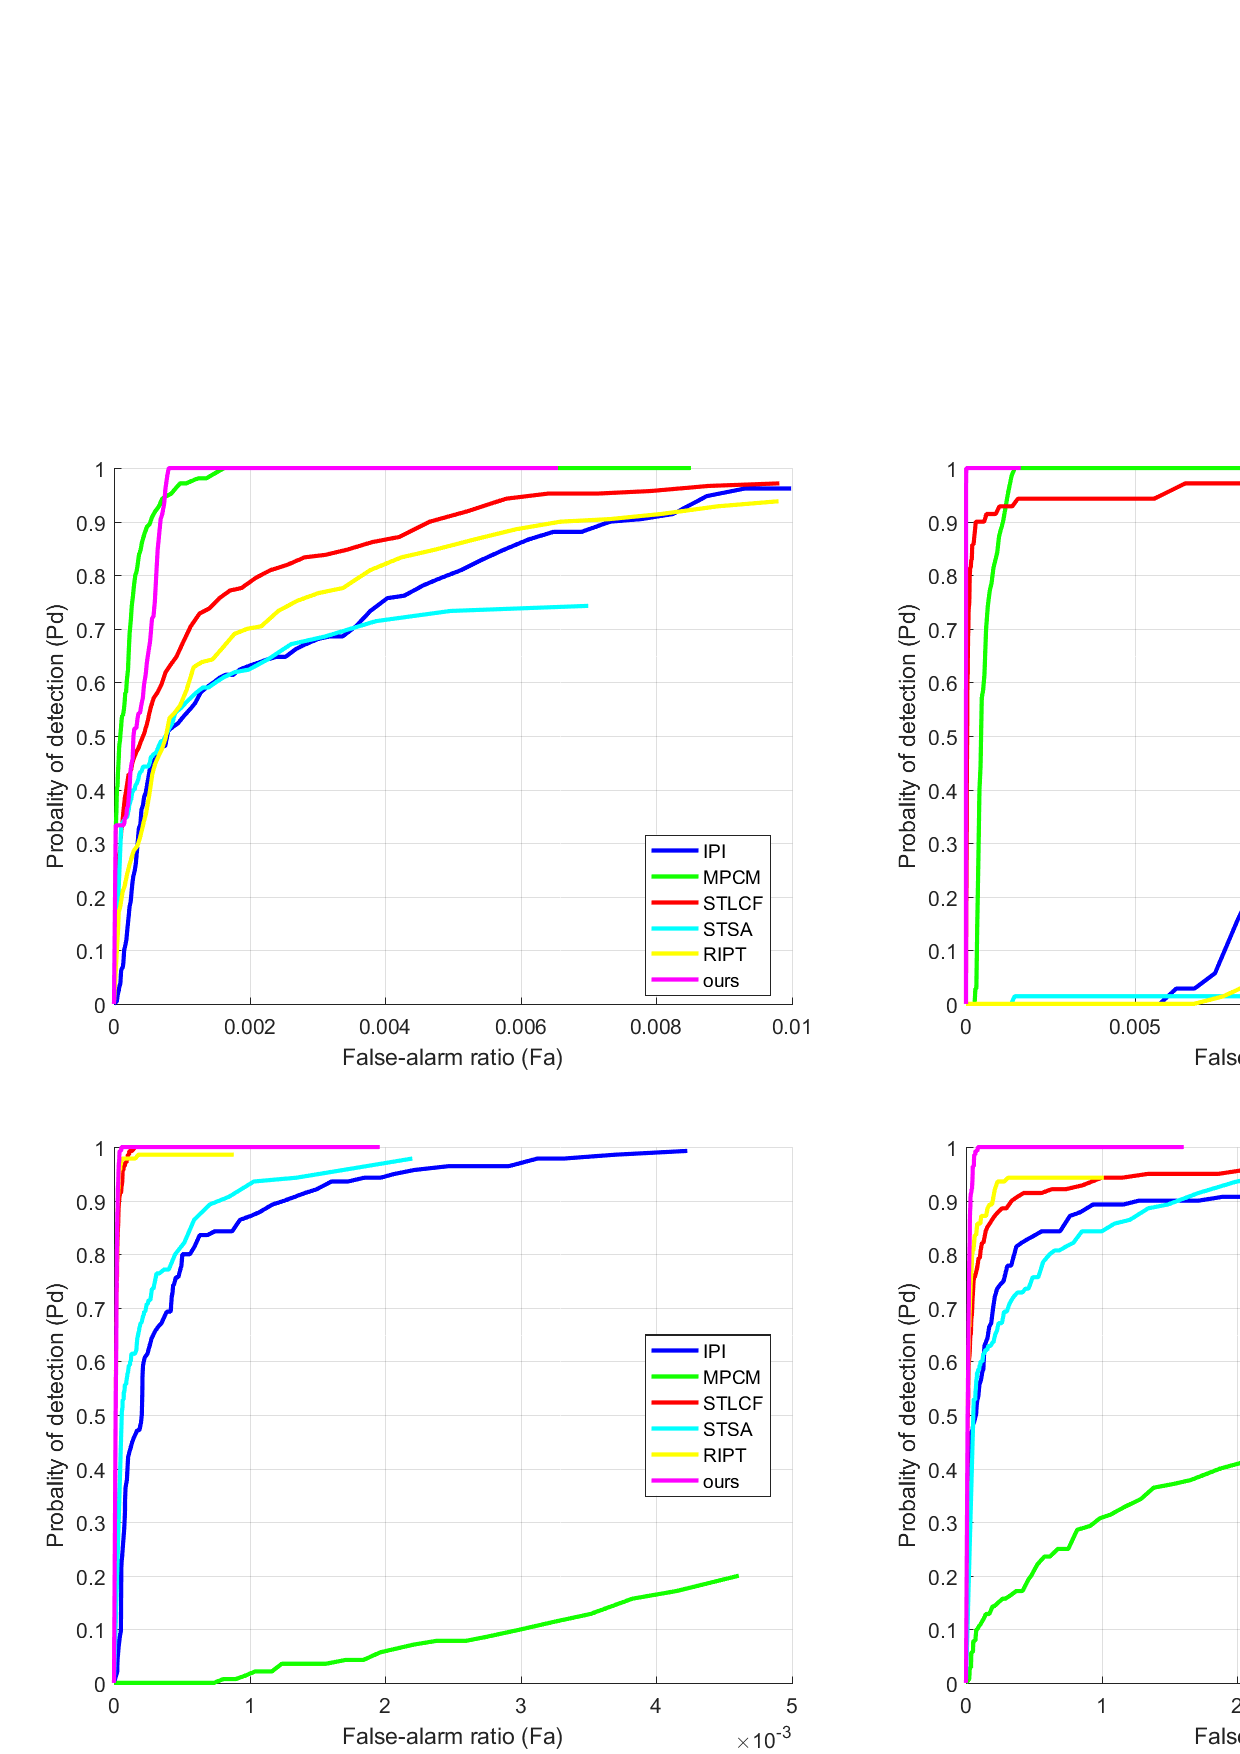
\includegraphics[width=0.95\textwidth]{ROC.pdf}
  \caption{First row: ROC curves on simulation video set. Second row: ROC curves on real video set.}
  \label{ROC}
\end{figure*}

\subsection{Comparsion of Detection Method on Infrared Video Set}
\subsubsection{Detection Results}
We performed six detection methods on different scenes of our video set. In order to show the detection results of different methods directly, we only show the detection results of the representative video frames mentioned in Table \ref{tab1} and \ref{tab2}. The detection results of six methods on simulation video set are shown in Figure \ref{result1}. And, the detection results of six methods on real video set are shown in Figure \ref{result2}.

It can be seen from Figure \ref{result1} that the methods including IPI, MPCM and RIPT have poor results on cloud plaques, building spots and other target-similar objects. And many plaque clutters exist common in target images obtained. Due to utilize spatial information only, the target-similar objects appearing in single image tend to be detected as true targets. So, the false alarm rate of these methods are higher then other methods. Then, the traditional methods based on local spatio-temporal contrast including STLCF and STSA, have bad results when dealing with moving background. There are many targets missed in the results obtained by STSA, as shown in Figure \ref{result1} seq1 and seq4. STLCF method is sensitive to pixel noise, so there is a lot of noise in the detection results, as shown in Figure \ref{result1} seq3 and seq4. Our method obtains better results on four sequences seen from Figure \ref{result1}.

It can be seen from Figure \ref{result2} that the methods including IPI and MPCM also view cloud plaques and bright spots of buildings as true targets mistakenly. Though RIPT can suppress strong edges effectively, it is difficult to recognize target-similar spots. Due to the noise of video is small and the movement of background is not obvious, STLCF and STSA have better results than single image based detectin methods, as shown in Figure \ref{result2} seq1 and seq2. But there are still small number of missed targets and false alarms in detection results. Howerer, it can be seen from Figure \ref{result2}, the method proposed by us has good results in four real videos.





\subsubsection{Measurement Metrics}
We also measure the results obtained from six detection methods via the metrics mentinoed above. The measurement metrics of simulation video set are shown in Table \ref{metrics1}. Meanwhile, the measurement metrics of real video set are shown in Table \ref{metrics2}.

It can be seen from above tables that our detection method has higher $\mbox{SCR}_{gain}$, $\mbox{LSNR}_{gain}$ and $\mbox{BSF}$. It proves that the method proposed by us can highlight target and suppress background better in infrared small target detection process. Some metrics corresponding to low-rank sparse tensor separation based methods including IPI, RIPT and our method are too large, even approaching infinity. It is common because of that the noise of background neighborhood is removed so that the standard deviation of noise in adjacent background region reduced to zero. In general, our method gets better measurement metrics than other methods.

\subsubsection{ROC Curve}
The ROC curves of six methods on infrared video set are given in Figure \ref{ROC}. It can be seen from Figure \ref{ROC} that the curves corresponding to our method always rise at the fastest speed, which means that our method can achieve the same accuracy as other methods with a smaller false alarm rate. Moreover, when the accuracy rate reaches maximum value, the false positive rate corresponding to our method is the smallest among all methods. It proves that the method proposed by us can effectively eliminate noise and avoid the influence of target-similar clutters. The ROC curves obtained by STSA method are usually at the bottom and raise slowly. The main reason for this phenomenon is that this method is greatly affected by noise and background motion. So, In the case of obvious noise, this method of image patch reconstruction is not feasible. And then, the curves of STLCF method raise significantly slower in scenes with large noise. Therefore, the false alarm rate of STLCF is much higher than other methods. It can also be seen from Figure \ref{ROC} that our method perform better than single image based methods including IPI, MPCM and RIPT due to the existence of cloud plaques, building sopts and other target-similar objects.


\section{Conclusion}
We propose an infrared small target detection method based on the spatio-temporal tensor model. The method can not only utilize the information in spatial domain to highlight target, but also can make full use of the context information in temporal domain to detect target more accurately. And our method performs good in different scenes.

Based on the method proposed in this paper, we need to slide a window continuously and construct spatio-temporal image patch cubes with image patches in spatio-temporal neighborhood. So, it is necessary costing much time to construct spatio-temporal tensors and obtain sparse tensors continuously. Therefore, our method runs slightly slow. Therefore, the next work is to optimize the method proposed in this paper and improve the detection speed further.





% if have a single appendix:
%\appendix[Proof of the Zonklar Equations]
% or
%\appendix  % for no appendix heading
% do not use \section anymore after \appendix, only \section*
% is possibly needed

% use appendices with more than one appendix
% then use \section to start each appendix
% you must declare a \section before using any
% \subsection or using \label (\appendices by itself
% starts a section numbered zero.)
%


\appendices
\section{Proof of the First Zonklar Equation}
Appendix one text goes here.

% use section* for acknowledgment
\section*{Acknowledgment}
The authors would like to thank...


% Can use something like this to put references on a page
% by themselves when using endfloat and the captionsoff option.
\ifCLASSOPTIONcaptionsoff
  \newpage
\fi



% trigger a \newpage just before the given reference
% number - used to balance the columns on the last page
% adjust value as needed - may need to be readjusted if
% the document is modified later
%\IEEEtriggeratref{8}
% The "triggered" command can be changed if desired:
%\IEEEtriggercmd{\enlargethispage{-5in}}

% references section

% can use a bibliography generated by BibTeX as a .bbl file
% BibTeX documentation can be easily obtained at:
% http://mirror.ctan.org/biblio/bibtex/contrib/doc/
% The IEEEtran BibTeX style support page is at:
% http://www.michaelshell.org/tex/ieeetran/bibtex/
%\bibliographystyle{IEEEtran}
% argument is your BibTeX string definitions and bibliography database(s)
%\bibliography{IEEEabrv,../bib/paper}
%
% <OR> manually copy in the resultant .bbl file
% set second argument of \begin to the number of references
% (used to reserve space for the reference number labels box)
\bibliographystyle{IEEEtran}
\bibliography{ref}
% biography section
%
% If you have an EPS/PDF photo (graphicx package needed) extra braces are
% needed around the contents of the optional argument to biography to prevent
% the LaTeX parser from getting confused when it sees the complicated
% \includegraphics command within an optional argument. (You could create
% your own custom macro containing the \includegraphics command to make things
% simpler here.)
\end{document}


